\chapter{工具实现与实验}\label{chapter_experiment}

\section{工具实现}

在上一章的方法中我们介绍了整体的优化框架一共分为4个不同的模块,分别是稳定性分析模块、计算路径提取模块、随机代数变换模块以及路径合并模块,在我们工具的实现中,每个模块都有对应的具体实现,其中路径提取模块以及随机代数变换模块存在一些技术难点,下面做具体介绍。

\subsection{基于KLEE符号执行的计算路径提取模块}

在这一模块中,我们通过符号执行的方式,将程序不稳定输入域上的计算路径提取出来。这一工作主要是基于符号执行技术来完成的,完全由自己手工来设计并实现一个符号执行工具将会是一项浩大的工程,因此我们选择对现有的符号执行工具进行改动,在其上添加新的功能以完成路径提取的工作。在这里我们选择KLEE\cite{Cadar:2008:KUA:1855741.1855756}作为我们的目标工具,KLEE本身是由斯坦福大学开发并发布的一个符号执行工具,其主要特点是能够通过符号执行的技术对复杂代码或者系统产生高覆盖率的测试用例。KLEE使用符号化的输入代替所有可能的具体的输入值,程序执行过程中的所有变量均会被表示成为关于这些符号化输入的表达式,并在遇到分支语句时构成对应路径的分支约束。从以上过程可以发现,KLEE能够完整的提供包括输入变量符号化,路径约束生产,符号执行等功能,因此我们选择在KLEE的基础上实现计算路径提取的功能。

然而,KLEE本身的功能并不完善,我们需要对KLEE进行改进以得到我们所需要的结果。我们主要对KLEE进行了以下改动,首先添加了对输出变量的识别功能,我们会在原数值计算程序中对需要输出的变量做类似于插桩的操作,将其标记为输出变量,表示我们需要在提取此变量关于程序输入的一个计算表达式,在KLEE的符号执行时,一旦遇到这样的变量,KLEE需要能够识别之,并在符号执行结束后在输出模块中将此变量对应的计算表达式输出。此外,我们的进行路径提取所得到的计算表达式中是必须能够包含一些基础的数学库函数的(比如sin、cos、ln函数等),然而KLEE在符号执行时却跳转入这些函数内部继续进行符号执行,这是我们不想看到的,为此,我们使KLEE在符号执行时有意的去忽略这些数学库函数,将其直接作为一个函数记录下来,而不是去做进一步的符号执行。最后是计算表达式的输出模块,在符号执行完成时,KLEE需要能够将需要的输出变量的计算表达式输出。

路径提取的结果最终会保存在一个路径文件中,对于如图\ref{lst:e_example_code}所示的使用泰勒级数近似计算自然对数e的数值计算程序,其对应抽取得到路径文件如图\ref{lst:e_example_pathfile}所示,路径文件中各个属性详细解释见表\ref{tab:pathfile_attributes}。


\begin{figure}[thbp]
    \begin{lstlisting}[%
      xleftmargin=7em,numberblanklines=true,boxpos=b,%,extendedchars=\true, %inputencoding=utf8%/latin1
      morekeywords={REAL, INTEGER}%keywords={main}
    ]
    REAL e_approx(INTEGER n) {
        REAL z = 2; 
        REAL y = 1;
        for (INTEGER i = 0; i < n; ++i) {
            y = y / i;
            z = z + y;
        }
        return z;
    }
    
    \end{lstlisting}
    %\vspace*{-4mm}
    \caption{泰勒级数近似计算自然对数$e$程序代码}
    \label{lst:e_example_code}
    %\vspace*{-4mm}
\end{figure}

\begin{table}[b]  
    \centering  
    \resizebox{\textwidth}{!}{
    \begin{tabular}{cl}  
      \\[-2mm]  
      \hline  
      \hline\\[-2mm]  
      {\bf \small 属性}  &   {\bf\small 含义}\\  
      \hline  
      \vspace{1mm}\\[-3mm]  
      program\_name     &   \tabincell{l}{程序名称}\\  
      \vspace{1mm}  
      function\_name    &   \tabincell{l}{函数名称}\\  
      \vspace{1mm}  
      variables         &   \tabincell{l}{所涉及到的变量及其对应类型}\\  
      \vspace{1mm}  
      intput\_variables &   \tabincell{l}{程序的输入变量}\\  
      \vspace{1mm}  
      output\_variables &   \tabincell{l}{程序的输出变量}\\  
      \vspace{1mm}  
      paths             &   \tabincell{l}{路径提取所得到的计算路径,为一个列表结构,列表中每个元素均为\\一个(约束,计算路径)二元组}\\  
      constrain         &   \tabincell{l}{计算路径对应的约束信息}\\  
      \vspace{1mm}  
      path              &   \tabincell{l}{一条计算路径,被抽象成为一个以procedure或是loop结构的列表的\\形式}\\  
      \vspace{1mm}  
      loops             &   \tabincell{l}{程序中涉及到的所有的循环信息}\\  
      \vspace{1mm}  
      loop\_body        &   \tabincell{l}{循环体信息,同样以计算路径的方式来表示,为一个列表结构,每个元\\素除了约束以及计算路径外,还附带了是否为循环出口的标记}\\  
      \vspace{1mm}  
      break             &   \tabincell{l}{循环体中的路径用来标记该路径是否为循环出口的标志}\\  
      \vspace{1mm}  
      procedures        &   \tabincell{l}{程序中所涉及到的所有的过程语句的信息,可以理解为顺序执行的一段\\代码,以列表形式给出,每个元素包含了变量及其对应计算形式信息}\\  
      \hline  
      \hline  
    \end{tabular}}
    \caption{路径文件属性说明表}  
    \label{tab:pathfile_attributes}  
\end{table} 



\begin{figure}[thbp]
\begin{lstlisting}[language=json,firstnumber=1]
{
    "program_name": "e_example",
    "function_name" : "e_approx",
    "variables" : {"n": "integer", "z": "decimal"},
    "input_variables": ["n"],
    "return": "z",
    "paths": [{
        "constrain": "true", 
        "path": ["procedure:p", "loop:l"]}],
    "loops": {
            "l": {
                "variables": {"i": "integer", "y": "decimal"},
                "initialize": {"i": "1", "y": "1.0"},
                "loop_body":[{
                    "constrain": "i<n",
                    "path": ["procedure:pp"],
                    "break": "false"
                    },
                    {
                    "constrain": "!(i<n)",
                    "path":[],
                    "break": "true"
                    }]
        }
    },
    "procedures": {
        "p": [["z", "1"]],
        "pp": [["y", "y/i"], ["z", "z+y"], ["i", "i+1"]]
    }
}
\end{lstlisting}
\caption{泰勒级数近似计算自然对数$e$程序路径文件}
\label{lst:e_example_pathfile}
\end{figure}

\subsection{基于规则模板的随机代数变换引擎}

在前面的章节我们介绍了一个基于规则库的随机代数变换方法,来寻找一个不稳定计算过程的等价稳定计算形式。随机代数变换的核心是转换规则库,为了能够方便我们灵活的添加与删除规则,我们实现了一个随机代数变换引擎,规则库以模板文件的形式给出,我们可以非常容易地在规则库中添加新的规则。该随机代数变换引擎主要使用到了ANTLR(Another Tool for Language Recognition)库,该库是一个语法解析器的生成器,我们首先需要定义模板文件的语法,ANTLR可以自动地帮助我们生成该语法对应的解析器。该解析器解析规则模板文件能够得到每一条规则对应的语法树结构,在整个语法树结构上,我们去完成原始表达式形式的匹配,如果匹配成功,我们则将原始表达式转换成为对应的转换后的计算形式。

模板文件每一条规则的语法如下所示:
 \begin{gather*}
    \text{rule\_name} : \text{origin\_expr} \rightarrow \text{transformed\_expr} @ \text{constrain}
 \end{gather*}

 其中rule\_name表示规则名称,origin\_expr表示转换前的计算表达式,也就是需要我们进行匹配的计算表达式,transfromed\_expr表示转换后的计算表达式,constrain表示进行这样的转换需要满足的约束。

\section{工具使用}

该数值程序优化工具在使用过程对用户非常友好,每一个模块的输出均会以文件的形式保存下来,用以提供给下一个模块作为输入使用,当想单独执行某几个模块时也可以选择性地执行,同时这样做也方便用户查看每个模块的中间结果。稳定性分析模块在执行结束后首先会生成一个json形式的以sa后缀结尾文件,里面存储了稳定性分析得到的结果,即原数值计算程序对应的稳定输入域,不稳定输入域信息。然后,路径提取模块对程序进行符号执行,提取程序的计算路径,将结果保存在一个以pth为后缀的路径文件中,具体形式上一小节已经作了具体介绍,在此不再赘述。紧接着,路径优化的模块会读取上个模块的输出,对其中的不稳定路径进行优化,得到的结果保存在opt.pth文件中,该文件结构与pth基本一致,只不过在文件中每条路径上新添加了具体的实现信息,以备后续路径合并时使用。最后,路径合并模块读取上一步的输出文件,将每条路径结合其实现信息组合成为最后的优化后程序。

在使用该工具之前,用户首先需要对工具进行一定的配置工作,所有的配置选项都保存在一个名为config.py的python文件中,下面对配置文件的选项做相关的介绍:

\texttt{MODULES = all, sa, pe, st, pm}\\
  执行模块设置。用户可以在配置文件中制定需要执行的模块,包括了sa(stable analysis)代表稳定性分析模块,pe(path extraction)代表了路径提取模块,sat(stochastic algebraic transformation)随机代数变换模块,pm(path merge)代表了路径合并模块,每个模块之间使用","分隔,同时用户也可以使用all这个配置选项来选择执行所有的模块。需要注意的是,前后模块之间有依赖关系,必须确保每个模块都有对应的输入文件才能选择执行,例如执行sat模块必须保证上一个模块的输出pth文件存在才能够执行,否则程序会报错。

\texttt{ERROR\_TOLERANCE = 3E-14\%}\\
  允许误差设置。该设置用于稳定性分析模块,代表了程序在进行稳定性分析时,能够所允许的任意精度程序与浮点精度程序在某一个输入域上的最大相对误差,超过这个误差,我们认为该输入域是不稳定的,若误差能够保证在这个范围以内,则我们认为该输入域为稳定的。IEEE754浮点数标准规定了,一个双精度浮点数由64个比特位组成,其中52位为有效数字位。因此,一个浮点数的基本表示误差在10-14\%左右。也就是说,就算我们仅仅对一个浮点数进行赋值操作,不考虑其他任何的计算操作,这样的赋值操作也有可能引入百分之1E-14的相对误差。因此我们一般将此设置项设置为3E-14\%,也就是说,当一个数值计算过程使用浮点数实现时,与其任意精度实现在某一输入域上的最大相对误差不超过3E-14\%时,我们便认为此输入域是稳定的。

\texttt{EXPR\_SETNUM = 100}\\
  等价代数集合设置。该设置表示在进行随机代数变换时,我们产生的等价代数集合的最大大小,一旦达到该大小然而还未寻找到稳定的计算形式,我们则结束搜索的过程,使用原任意精度的数值计算过程。

\texttt{TIMEOUT = 10min}\\
  随机代数变换超时设置。该设置表示在进行随机代数变换时,允许的最大搜索时间,一旦超时,我们同样的也会结束整个搜索过程,使用原任意精度的数值计算过程。


在完成了上述的相关配置后,用户便可以直接执行优化程序,将原程序代码的文件路径作为命令行参数给出,在完成优化后在同目录下会生成多个中间结果的文件,以及最终的优化后的以opt.cc结尾的代码文件。

\section{实验}

为了验证我们的工具的有效性,我们进行了两部分实验:实验一的实验对象是iRRAM任意精度数值计算库的中典型的数值计算程序,进行了数值计算程序在优化前后的运行结果以及运行效率的对比,旨在说明我们的优化工具能够在保证数值程序正确性的前提下大幅度地提高数值程序的运行效率。在实验二中,我们选取了GNU科学计算库中一些常用的数学函数,我们自己实现了一套这些数学函数的任意精度版本,并使用我们的优化框架对其进行了优化,然后与GNU科学计算库中的代码实现进行了一系列比较,主要说明了我们的优化工具能够帮助软件开发人员更容易地开发易读易维护且正确高效的数值计算程序。

两次实验使用的电脑为Dell Workstation Precision T1700,处理器为Intel(R) Core(TM) i7-4790@3.60GHz 8核处理器,内存16GB,操作系统为Ubuntu 14.04LTS,使用系统默认编译器gcc4.8.0。

\subsection{iRRAM任意精度程序优化实验}

为了说明我们的优化工具可以在保证数值程序正确性的前提下大幅度的提升数值程序的运行效率,我们进行了iRRAM任意精度程序优化实验。我们选取了iRRAM任意精度数值计算库中的部分数值计算程序,对这些数值计算程序进行了优化。我们主要考察了每个数值计算程序在优化前后程序运行结果与正确结果的差异以及在运行时间上的变换情况。实验结果表明,经过我们优化工具优化后的数值程序,其计算结果与正确的任意精度程序基本保持一致,同时其运行效率得到了大幅度的提升。

为了在版本迭代时能够方便地进行测试,iRRAM任意精度数值计算库的源码中附带了一系列数值计算程序,这些数值计算程序由任意精度编写,并且囊括了许多经典的数值计算问题。我们对这些程序进行了筛选,去除掉了一些与数值计算问题无关的测试程序(比如直接将一个字符串转换为数值类型的测试程序)选出了11个数值计算程序作为我们待优化的目标程序,表\ref{tab:irram_examples}简要展示了每个数值程序的具体计算内容。

\begin{table}[h]  
    \centering  
    \begin{tabular}{cl}  
      \hline  
      \hline\\[-1mm]  
      {\bf \small 程序}  &   {\bf\small 说明}\\  
      \hline  
      \vspace{1mm}\\[-3mm]  
      analytic     &   \tabincell{l}{以一个简单算法计算$1/2^{20}$的计算程序}\\  
      \vspace{1mm}  
      e\_example    &   \tabincell{l}{使用级数$\sum_{i=0}^{n}1/i!$计算自然对数$e=2.71828...$}\\  
      \vspace{1mm}  
      float\_extension &   \tabincell{l}{计算$2+\sum_{i=1}^{100,000}1/\sqrt{i}$的数值计算程序}\\  
      \vspace{1mm}  
      gamma\_bernoulli &   \tabincell{l}{使用斯特林方法近似计算欧拉常数$\gamma = 0.577...$}\\  
      \vspace{1mm}  
      harmonic &   \tabincell{l}{计算调和级数\cite{HOFFMAN1997477}的前$n$项和}\\  
      \vspace{1mm}  
      itsyst  & \\
      itsyst2 &   \tabincell{l}{以不同的输入迭代计算$x_{i+1} = 3.75x_i(1-x_i)$\cite{SPANDL20121459}}\\  
      itsyst3 &  \\
      \vspace{1mm}  
      jmmuller &   \tabincell{l}{以不同输入迭代计算$x_{i+2}=3000/(1130-x_i(111-x_{i-1})$\cite{muller:ensl-00086707}}\\  
      jmmuller2 &  \\
      \vspace{1mm}  
      lambov &   \tabincell{l}{计算泰勒余项\cite{Radzievskaya2003}}\\  
      \hline  
      \hline  
    \end{tabular}  
    \caption{iRRAM示例程序说明表}  
    \label{tab:irram_examples}  
\end{table} 

对于每个计算程序,我们对比了以下三个不同版本的程序代码的运行结果以及运行效率:

{\kaishu 原iRRAM库中的任意精度程序:} 
iRRAM任意精度库自带的示例程序,这些数值程序使用任意精度类型的实现,能够保证绝对的正确性,并且在计算资源允许的情况下,对于每一个数值计算程序,其可以输出任意多位的有效数字。由于使用了任意精度类型进行计算,这一版本的数值程序能够保证其输出是绝对正确的,我们将这样的程序作为标杆程序,即所有与正确结果的比较实际上都是与这些程序的输出进行的比较。而正如我们在前文中所提到的,任意精度计算在保证程序正确性的代价是占用更多的计算资源,从后面的实验表格中我们也可以看出,这样的任意精度程序虽然计算结果完全正确,但是其与普通浮点精度的计算效率差别显著,浮点精度计算效率明显的高于任意精度计算。

{\kaishu 相同计算过程的浮点精度程序:} 
为了体现我们优化工作的意义所在,我们在设计实验时添加了这样的程序,这些程序与iRRAM任意精度程序的计算过程是完全相同,然而计算中使用的精度都由iRRAM的任意精度类型REAL转换为了普通的双精度浮点类型double,同时函数调用也进行了转换,所有任意精度的数学函数调用也被转换为了普通浮点精度对应的函数调用。一个普通的软件开发人员在开发数值程序时,如果直接按照软件需求使用浮点精度来进行程序开发得到的便是这样的程序,从后面的实验结果中我们可以看出,这样的程序在绝大多数情况下都会产生非常大的误差。 

{\kaishu 优化工具优化后程序:} 
我们将原任意精度程序作为输入,交给我们的优化工具,得到的优化后程序。原来的任意精度的数值程序的计算过程是不稳定的,因此才会有相同计算过程的浮点精度程序的计算结果与正确值相差非常大的情况。在经过我们的优化工具进行优化后,这些不稳定的计算过程被我们的优化工具替换为了在数学上等价的稳定的计算过程,并且使用浮点精度实现成为我们优化后的程序。这样的优化后的程序既保证了程序的正确性,同时程序的计算效率也与浮点精度类型的数值程序没有多少差异。

\begin{table*}[thbp]
   \centering
   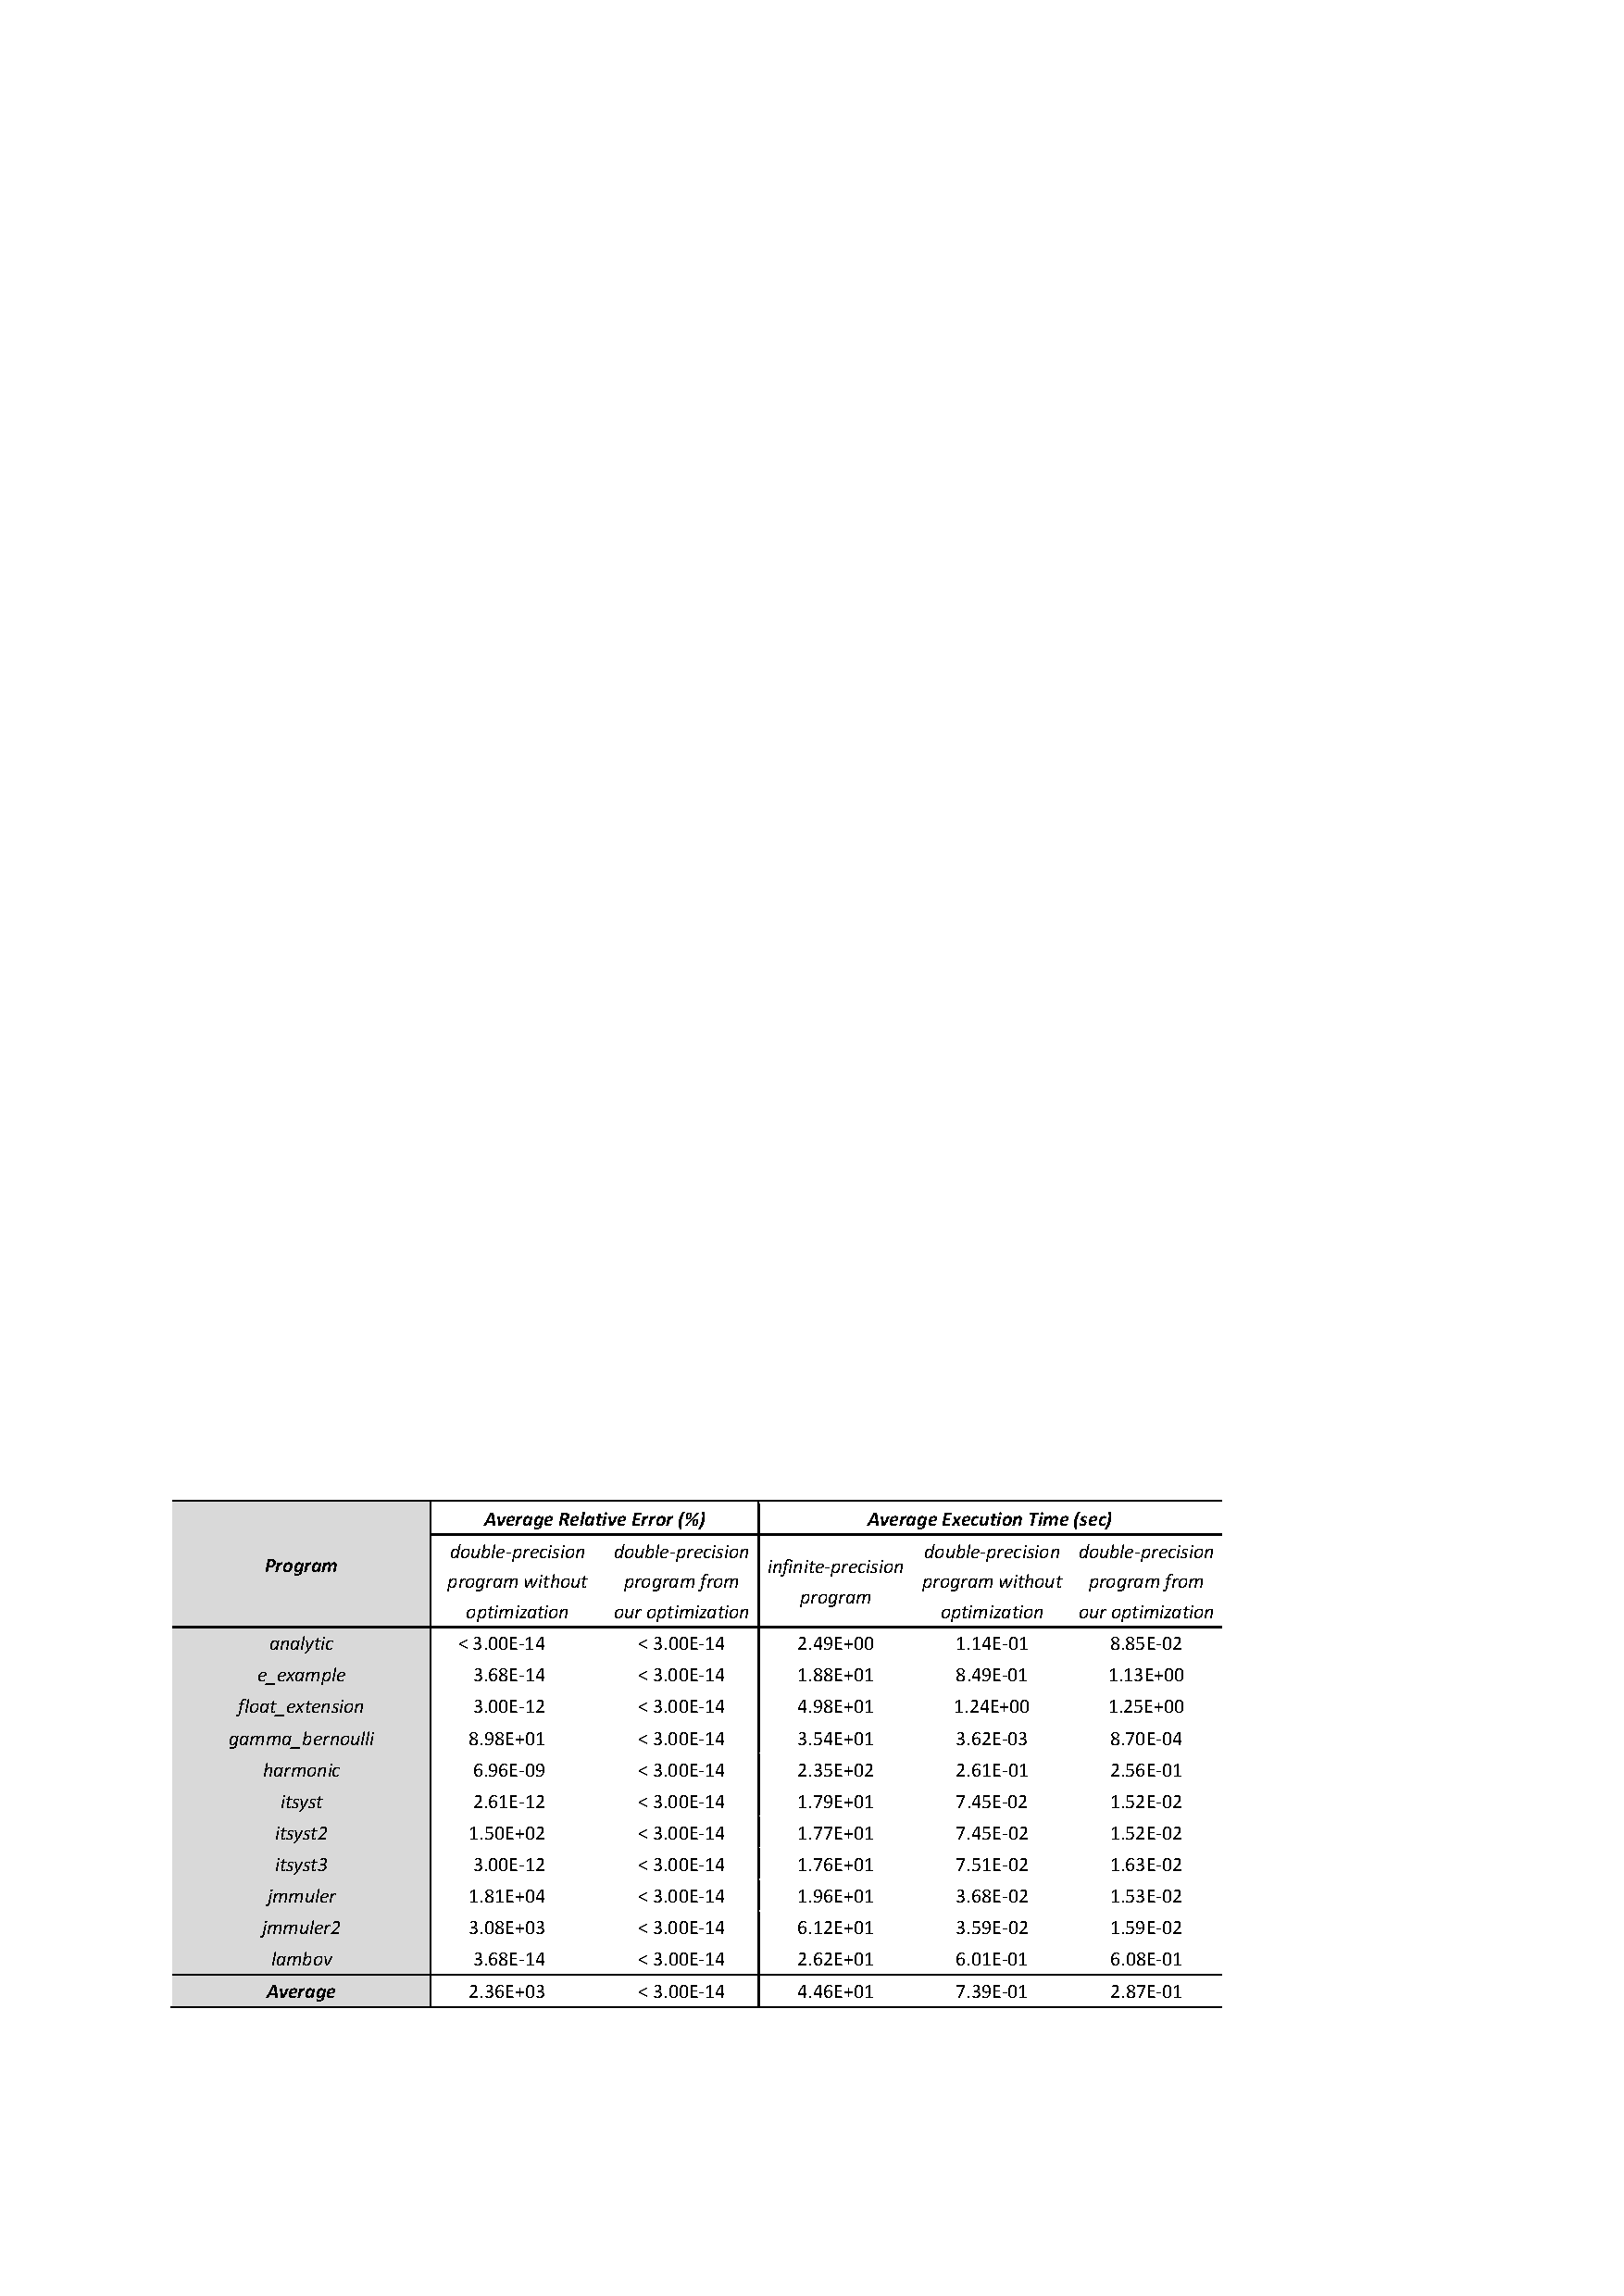
\includegraphics[width=\columnwidth]{fig/EvalTable_ErrorTime.pdf}
   \caption{iRRAM示例程序误差即运行时间表} \label{fig:error_time}
\end{table*}

实验一的实验结果如表\ref{fig:error_time}所示,每个实验用例的第一行、第二行、第三行分别对应了iRRAM任意精度版本,浮点精度版本以及优化工具优化后版本。
从实验结果中我们可以看到,所有优化工具优化后版本的程序输出与正确结果的相对误差均不超过$3 \times 10^{-14}\%$,我们在上一小节实验设置中容许误差中讨论到,当一个浮点精度的计算程序与正确结果的相对误差不超过$3 \times 10^{-14}\%$时,我们可以认为这个浮点精度的计算过程是计算稳定的,因此我们可以认为经过我们优化工具优化后的数值程序均计算稳定。作为对比,相同计算过程的浮点双精度版本的程序的计算结果与正确结果差异非常大,只有少数程序如analytic、e\_example以及lambov其计算过程本身便是稳定的,对于其他任意精度的数值计算程序来说,如果直接使用浮点双精度类型来实现相同的计算过程,其计算结果与正确结果最多可以相差几万倍,其平均的相对误差也达到了$2.36 \times 10^{3}\%$。从这一实验结果我们可以得出结论,经过我们优化工具优化得到的优化后程序保持了原任意精度计算程序的正确性。

除了比较程序的运行结果,我们同时也比较了三种不同程序运行时间。从表中可以看到,原任意精度程序的平均运行时间为45.62秒,然而直接的浮点精度程序以及我们优化后的程序的平均运行时间分别为0.306秒和0.310秒,对于绝大对数任意精度程序来说,其运行时间是相同计算过程的浮点精度程序的几百甚至几千倍,由此可见,任意精度程序的执行效率是非常低下的。同时,我们也观察到,我们优化工具优化后的程序的运行效率部分高于浮点精度版本,部分低于浮点精度版本,但是在总体上与浮点精度版本基本保持一致。这样的结果也是在我们的预期之中的,产生这样的现象的原因是由于我们优化工具找到的等价计算过程的复杂程度不是确定的,有时我们能够找到更加简单的稳定的计算过程,有时生成的优化后程序会包含非常复杂的路径判断,同时找到的稳定的等价的计算过程也有可能很复杂,导致了程序运行效率相较于浮点精度版本更为低下。但是总体来说,经过我们优化工具优化后得到的优化后程序的运行效率总体与相同计算过程的浮点精度版本保持一致,远远高于原来的任意精度版本的数值程序。这一实验结果表明,我们的优化工具能够大幅度提升原任意精度数值程序。

综合上述两点实验结果的分析我们可以得出结论,经过我们优化工具优化后的数值程序,在保证了正确性的前提下,大幅提升了程序的执行效率。


\subsection{GNU科学计算库函数实现实验}

为了说明我们的优化工具能够帮助软件开发人员更加简单更加容易地开发数值程序,我们进行了GNU科学计算库函数实现的实验。前文中我们提到,使用我们的优化工具,即便不具备专业的数值计算背景知识,软件开发人员也能够开发出正确并且高效的数值程序,因为软件开发人员只需要按照软件需求中的数学公式来编写数值计算程序的代码,而不用考虑复杂的误差控制以及与精度相关的操作。我们以GNU科学计算库中的部分常用的数学函数为实验目标,要开发这样的数学函数的数值程序,一种方法便是像GNU科学计算库一样,使用浮点精度来进行编程,其中掺杂了非常复杂的浮点数处理的技巧,这样进行开发得到的代码是非常复杂并且难以阅读难以维护的,另一种开发方式便是使用我们的优化工具进行开发,直接按照数学上的公式使用任意精度类型来编写程序,然后交给我们的优化工具进行优化,得到最终的优化后程序。在这一实验中,我们比较了这两种不同的开发方式所得到的代码的各种软件度量指标,实验结果表明,使用我们的优化工具进行开发可以使得开发过程更加简单,代码也易于理解和维护。

我们使用了业界常用的几种软件度量标准,包括了霍尔斯特德复杂度\cite{1702603}\cite{Bailey:1981:SSU:1010627.807928}、圈复杂度\cite{1702388}\cite{106988}以及可维护性指数\cite{Heitlager:2007:PMM:1306876.1307252}。

霍尔斯特德复杂度是由霍尔斯特德在1977年提出的一种软件度量标准,其主要是依据程序源代码中的运算符和操作数来衡量源程序代码的复杂程度。在霍尔斯特德复杂度度量方法中,运算符是指用来处理程序中常量和变量的语法元素等,如算术运算符、逻辑运算符、关系运算符、流程控制语句、函数调用等;操作数则是指源程序代码中的常量和变量等,但对非执行语句,如注释,则不进行考虑。Halstead方法使用了以下4个基本测量数据:

\begin{table}[h]  
    \centering  
    \begin{tabular}{|p{5cm}<{\centering}|p{3cm}<{\centering}|}  
      \hline  
      程序中运算符总数 &   $N_1$\\
      \hline  
      程序中操作数总数 &   $N_2$\\  
      \hline  
      程序中运算符种类数 &   $n_1$ \\  
      \hline  
      程序中操作数种类数 &  $n_2$\\  
      \hline  
    \end{tabular}  
\end{table} 

根据以上4个测量数据,可以在以下几个方面对源程序代码的复杂性进行度量:

\begin{table}[h]  
    \centering  
    \begin{tabular}{|p{5cm}<{\centering}|p{5cm}<{\centering}|}  
      \hline  
      程序长度 &   $N = N_1 + N_2$\\
      \hline  
      程序词汇数 &   $n = n_1 + n_2$\\  
      \hline  
      计算程序长度 &  $ \hat{N} = n_1 \log{n_1} + n_2 \log{n_2}$ \\  
      \hline  
      程序容量 &  $V = N \log{n}$\\  
      \hline  
      程序难度 &  $ D = \frac{n_1}{2} \times \frac{N_2}{n_2}$\\  
      \hline  
      程序精力 &  $ E = D \times V$\\  
      \hline  
    \end{tabular}  
\end{table} 

在本次实验中,我们使用了程序容量$V$这一度量指标,这一指标代表了写一个程序所需的信息量,越高则表明该程序越难以开发和维护。

圈复杂度也被称作条件复杂度或是循环复杂度,是另一种代码复杂程度的衡量标准,是由 Thomas J. McCabezz,Sr. 在 1976 年提出,圈复杂度是对源代码中线性独立路径数的定量测量。

圈复杂度由程序的控制流图\cite{Allen:1970:CFA:390013.808479}来计算,程序的控制流图是一个有向图,图中的节点为程序的基础模块,若一个模块结束后,可能会运行另一个模块,则用箭头链接二个模块,并标示可能的运行顺序。程序的圈复杂度由以下公式来计算:
\begin{align*}
    C = E - X + 2P
\end{align*}

其中 E 为图中边的个数, X 为图中节点的个数,P 为连接组件的个数。圈复杂度高说明程序代码的判断逻辑复杂,代码质量越低且更加难以测试和维护。

可维护性指数是一个结合了霍尔斯特德复杂度,圈复杂度以及代码行数的综合性指标,其计算公式如下所示:
\begin{align*}
    MI = 171 - 5.2\ln V - 0.23C - 16.2\ln LOC + 50\sin\sqrt{2.46CM}
\end{align*}

其中V代表了程序容量,C代表了程序圈复杂度,LOC代表了代码行数,CM代表了程序中的注释占总程序量的百分比,由于我们只考虑数学函数数值计算程序的具体代码实现,所以我们忽略计算公式中的CM。可维护性指数越高,表明程序越易于维护。

\begin{table*}[thbp]
    \centering
    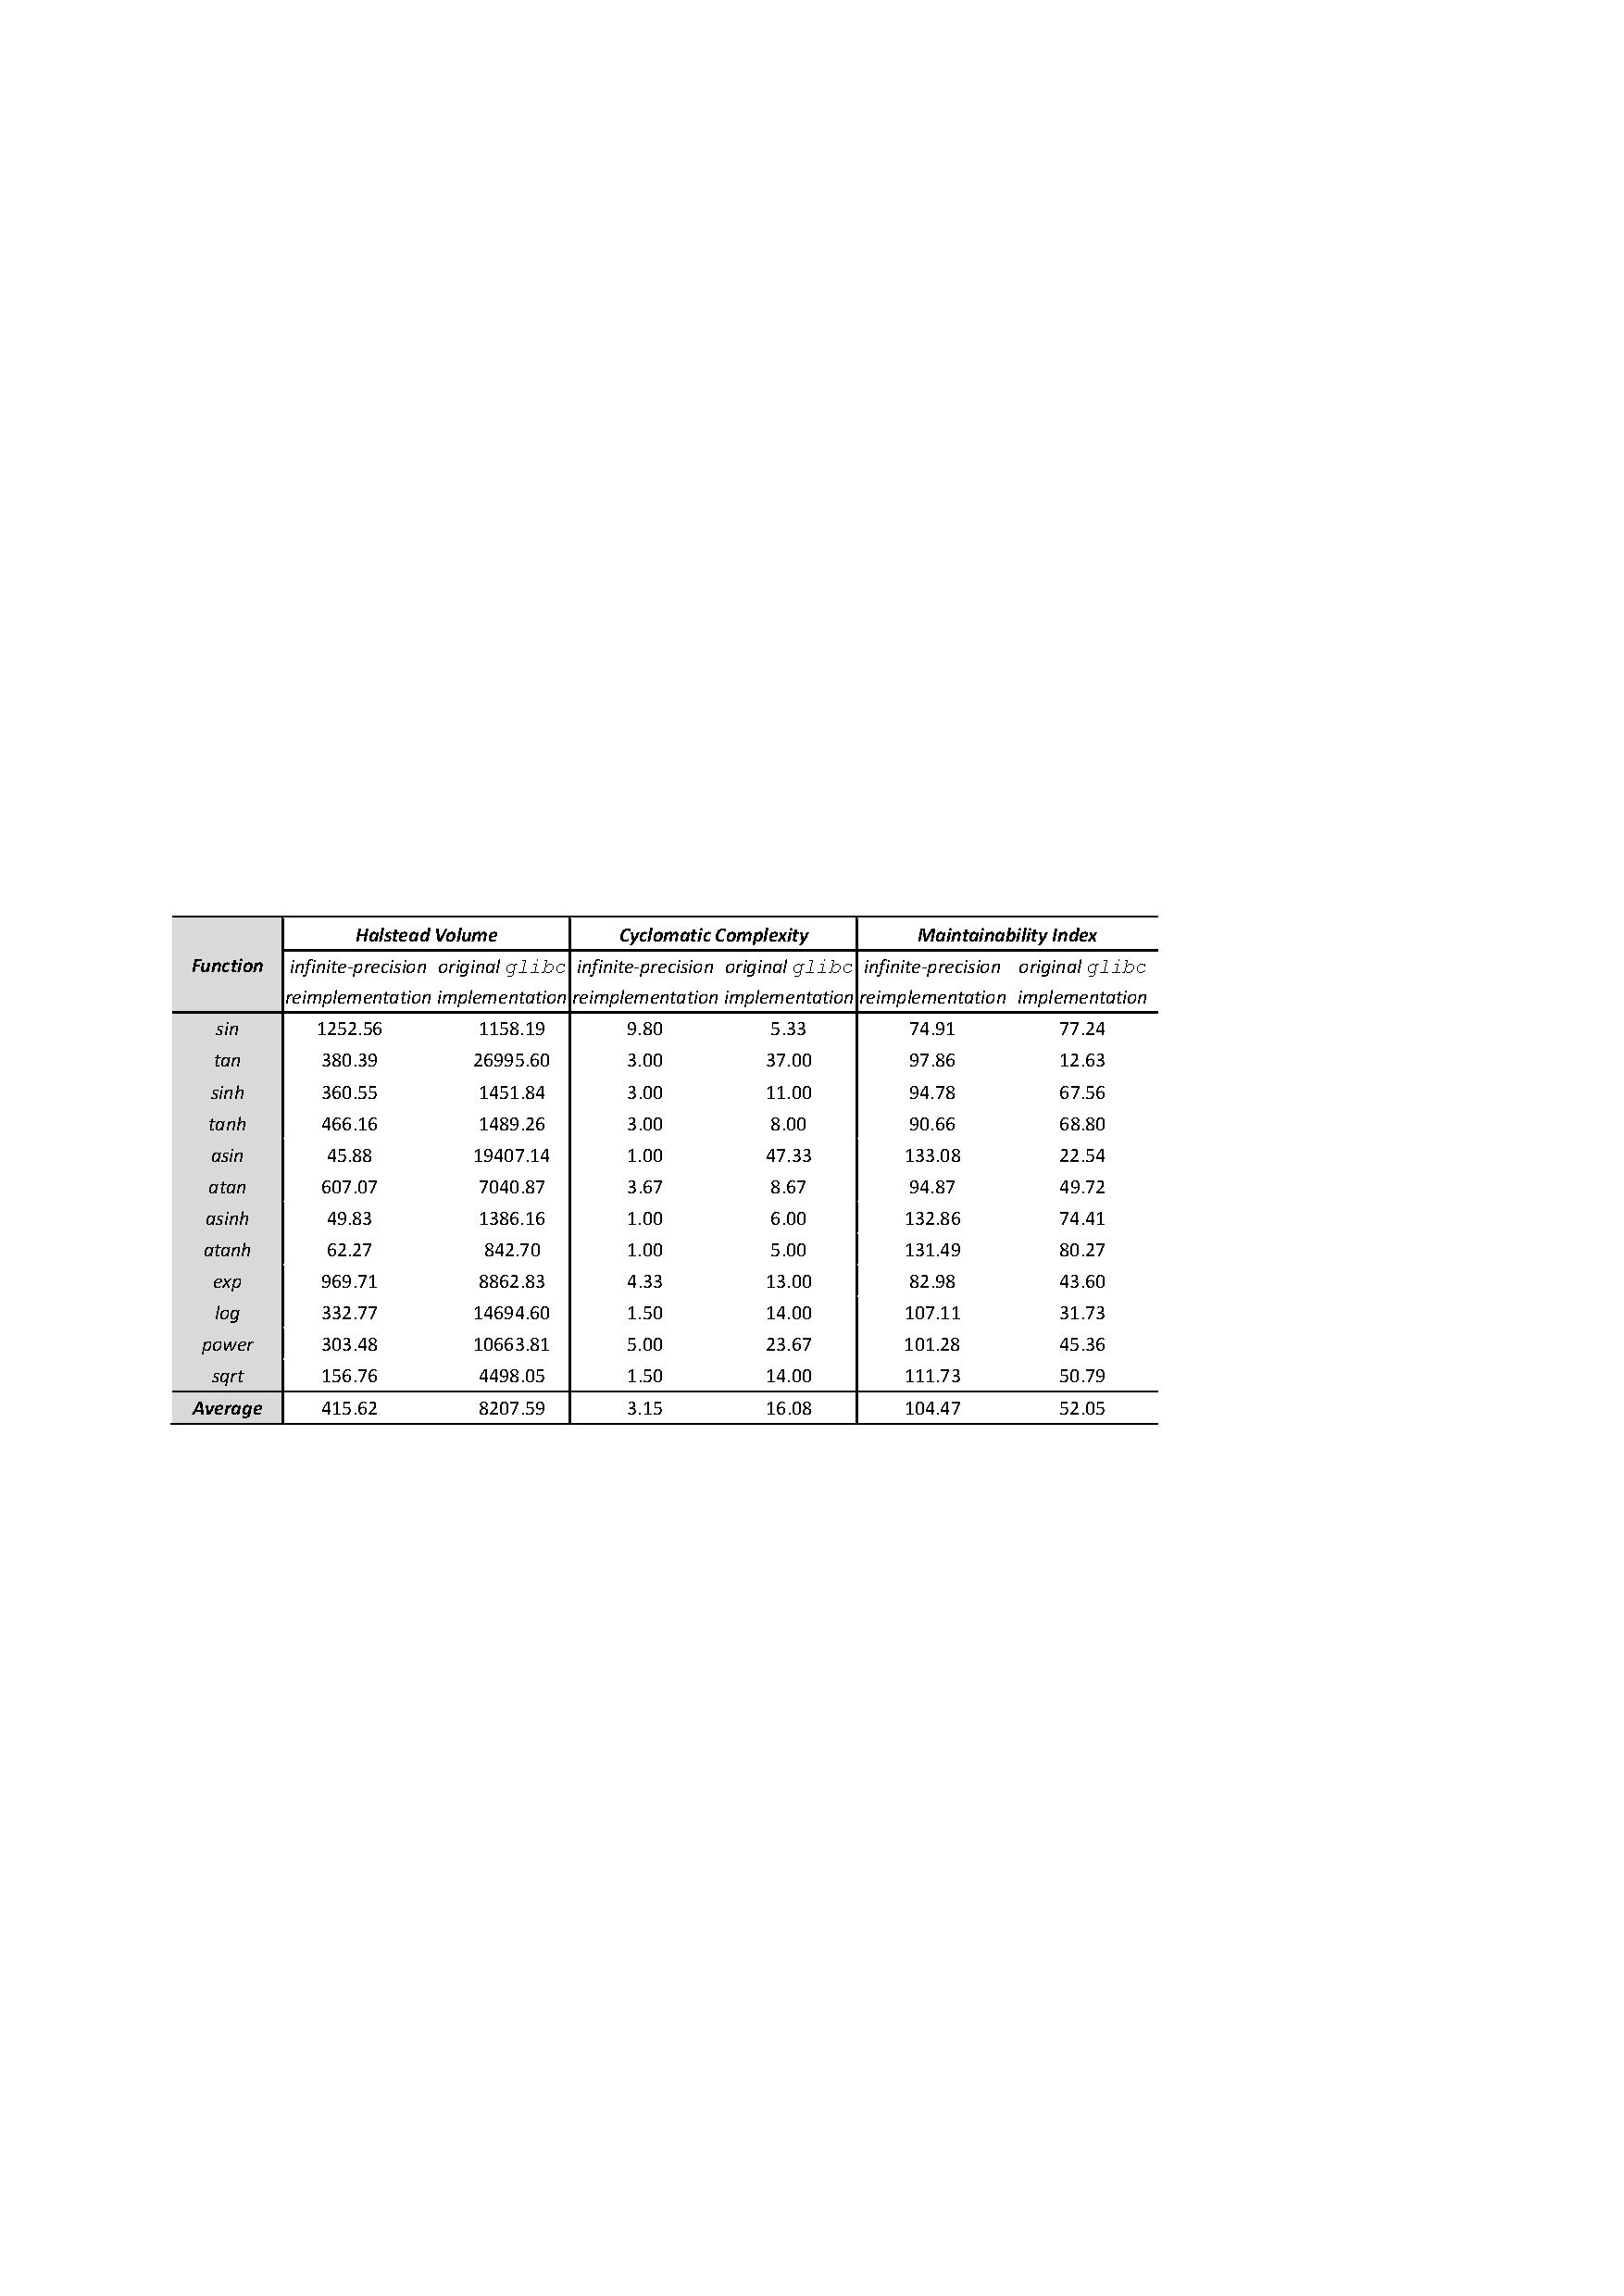
\includegraphics[width=\columnwidth]{fig/EvalTable_ComplexMeasurements.pdf}
    \caption{GNU库函数在度量指标对比表} \label{fig:complex_measurements}
 \end{table*}

表\ref{fig:complex_measurements}展示了两种不同实现的个度量指标的对比,某些函数使用了大量相同的代码实现,其各项度量指标基本保持一致,因此我们在这里只列举了其中的一个(例如sin函数与cos函数)。从表格中我们可以观察到,GNU科学计算库在实现浮点精度的数值计算程序时引入了大量的精度相关的操作,导致其函数实现相比于我们使用任意精度实现的代码复杂了很多。任意精度代码的平均程序容量大概只有浮点精度代码的二十分之一,这样的结果表明开发浮点精度代码需要的信息量大概是开发任意精度代码的20倍,可见软件开发人员需要更多相关的专业知识才能完成浮点精度程序的开发工作。再看两种不同版本的实现在圈复杂度上的表现,任意精度程序的圈复杂度也仅仅只有浮点精度程序的五分之一,该结果表明任意精度程序中独立的计算路径的数量大概为浮点精度程序的五分之一,说明任意精度程序代码的复杂程序远远地低于浮点精度程序。在综合指标可维护性指数上,任意精度实现的平均可维护性指为104.47,是浮点精度实现的两倍左右,说明了任意精度代码比浮点精度代码更加的易于维护。从上述实验结果我们可以看出,使用任意精度编写代码,然后使用优化框架进行优化这样的开发数值计算程序的开发方式比直接使用浮点精度代码进行开发能够使程序更加简洁,具有更高的可读性与可维护性。与此同时,程序员即便不具备数值计算专家的专业知识,也能够开发出高效正确的数值计算代码。

\section{本章小结}

在本章中,我们基于上一章节中提到的数值程序的优化方法,实现了一个数值计算程序的优化工具,并具体介绍了一些重点的模块,包括基于KLEE符号执行完成的路径提取模块,基于规则模板的随机代数变换引擎等。

随后我们进一步的说明了工具的使用方法,使用工具时各个配置项的具体含义。为了验证我们的工具在对于现实世界中的数值计算程序的优化效果,我们选取了iRRAM高精度数值计算库中的一系列测试程序进行了优化。结果表明,我们的工具能够在不影响程序正确性的情况下极大地提升数值计算程序的运行效率。而后,为了说明我们的工具能够帮助软件开发人员更加轻松地开发高效正确的数值计算代码,我们选取了GNU科学计算库中部分常用的数学函数,比较了直接的浮点精度实现以及任意精度实现在各个度量指标上的表现,证明了我们的工具的确可以极大提升软件开发人员在开发数值计算程序时的开发效率,同时也能够使得数值计算程序更加易读易维护。